% Options for packages loaded elsewhere
\PassOptionsToPackage{unicode}{hyperref}
\PassOptionsToPackage{hyphens}{url}
%
\documentclass[
  ignorenonframetext,
]{beamer}
\usepackage{pgfpages}
\setbeamertemplate{caption}[numbered]
\setbeamertemplate{caption label separator}{: }
\setbeamercolor{caption name}{fg=normal text.fg}
\beamertemplatenavigationsymbolsempty
% Prevent slide breaks in the middle of a paragraph
\widowpenalties 1 10000
\raggedbottom
\setbeamertemplate{part page}{
  \centering
  \begin{beamercolorbox}[sep=16pt,center]{part title}
    \usebeamerfont{part title}\insertpart\par
  \end{beamercolorbox}
}
\setbeamertemplate{section page}{
  \centering
  \begin{beamercolorbox}[sep=12pt,center]{part title}
    \usebeamerfont{section title}\insertsection\par
  \end{beamercolorbox}
}
\setbeamertemplate{subsection page}{
  \centering
  \begin{beamercolorbox}[sep=8pt,center]{part title}
    \usebeamerfont{subsection title}\insertsubsection\par
  \end{beamercolorbox}
}
\AtBeginPart{
  \frame{\partpage}
}
\AtBeginSection{
  \ifbibliography
  \else
    \frame{\sectionpage}
  \fi
}
\AtBeginSubsection{
  \frame{\subsectionpage}
}
\usepackage{amsmath,amssymb}
\usepackage{iftex}
\ifPDFTeX
  \usepackage[T1]{fontenc}
  \usepackage[utf8]{inputenc}
  \usepackage{textcomp} % provide euro and other symbols
\else % if luatex or xetex
  \usepackage{unicode-math} % this also loads fontspec
  \defaultfontfeatures{Scale=MatchLowercase}
  \defaultfontfeatures[\rmfamily]{Ligatures=TeX,Scale=1}
\fi
\usepackage{lmodern}
\usetheme[]{metropolis}
\usecolortheme{seahorse}
\ifPDFTeX\else
  % xetex/luatex font selection
\fi
% Use upquote if available, for straight quotes in verbatim environments
\IfFileExists{upquote.sty}{\usepackage{upquote}}{}
\IfFileExists{microtype.sty}{% use microtype if available
  \usepackage[]{microtype}
  \UseMicrotypeSet[protrusion]{basicmath} % disable protrusion for tt fonts
}{}
\makeatletter
\@ifundefined{KOMAClassName}{% if non-KOMA class
  \IfFileExists{parskip.sty}{%
    \usepackage{parskip}
  }{% else
    \setlength{\parindent}{0pt}
    \setlength{\parskip}{6pt plus 2pt minus 1pt}}
}{% if KOMA class
  \KOMAoptions{parskip=half}}
\makeatother
\usepackage{xcolor}
\newif\ifbibliography
\usepackage{graphicx}
\makeatletter
\def\maxwidth{\ifdim\Gin@nat@width>\linewidth\linewidth\else\Gin@nat@width\fi}
\def\maxheight{\ifdim\Gin@nat@height>\textheight\textheight\else\Gin@nat@height\fi}
\makeatother
% Scale images if necessary, so that they will not overflow the page
% margins by default, and it is still possible to overwrite the defaults
% using explicit options in \includegraphics[width, height, ...]{}
\setkeys{Gin}{width=\maxwidth,height=\maxheight,keepaspectratio}
% Set default figure placement to htbp
\makeatletter
\def\fps@figure{htbp}
\makeatother
\setlength{\emergencystretch}{3em} % prevent overfull lines
\providecommand{\tightlist}{%
  \setlength{\itemsep}{0pt}\setlength{\parskip}{0pt}}
\setcounter{secnumdepth}{-\maxdimen} % remove section numbering
\usepackage{xcolor}
\definecolor{myorange}{RGB}{255, 94, 77}
\ifLuaTeX
  \usepackage{selnolig}  % disable illegal ligatures
\fi
\IfFileExists{bookmark.sty}{\usepackage{bookmark}}{\usepackage{hyperref}}
\IfFileExists{xurl.sty}{\usepackage{xurl}}{} % add URL line breaks if available
\urlstyle{same}
\hypersetup{
  pdftitle={Graphical Excellence},
  pdfauthor={(\textbackslash text\{Professor Dave\})\^{}2},
  hidelinks,
  pdfcreator={LaTeX via pandoc}}

\title{Graphical Excellence}
\author{\((\text{Professor Dave})^2\)}
\date{}

\begin{document}
\frame{\titlepage}

\begin{frame}{Outline}
\protect\hypertarget{outline}{}
\emph{The Visual Display of Quantitative Information} provides a rich
story of graph types and excellence including:

\begin{itemize}
\item
  What is excellence?
\item
  Data maps
\item
  Time series
\item
  Space-time narrative designs
\item
  Relational graphics
\item
  Some history
\end{itemize}
\end{frame}

\begin{frame}{How is excellence achieved?}
\protect\hypertarget{how-is-excellence-achieved}{}
When complex ideas are expressed with:

\begin{itemize}
\item
  Clarity
\item
  Precision
\item
  Efficiency
\end{itemize}

\vspace{4mm}
\pause

How do we get there?

\begin{itemize}
\item
  \textcolor{orange}{Do}: Show the data clearly, aim to have a quick
  understanding of the data trend, facilitate comparisons.
\item
  \textcolor{orange}{Don't}: Distort the data, compress data in small
  spaces, show data at different scales.
\end{itemize}
\end{frame}

\begin{frame}{Why visualize? \textcolor{orange}{Anscombe's Quartet}}
\protect\hypertarget{why-visualize}{}
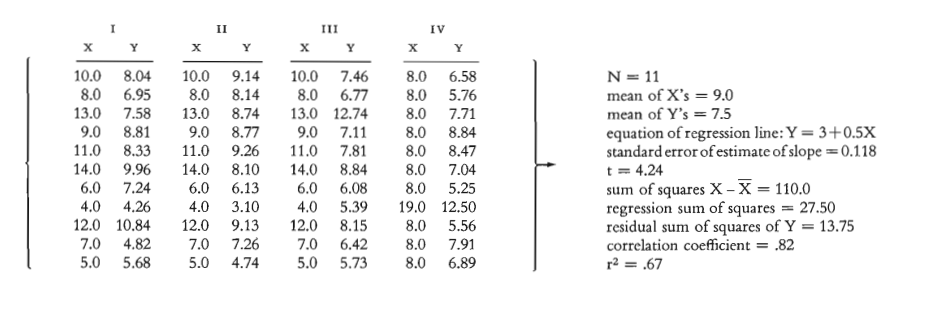
\includegraphics{excellence_figs/fig_1.png}
\end{frame}

\begin{frame}{Why visualize? \textcolor{orange}{Anscombe's Quartet}}
\protect\hypertarget{why-visualize-1}{}
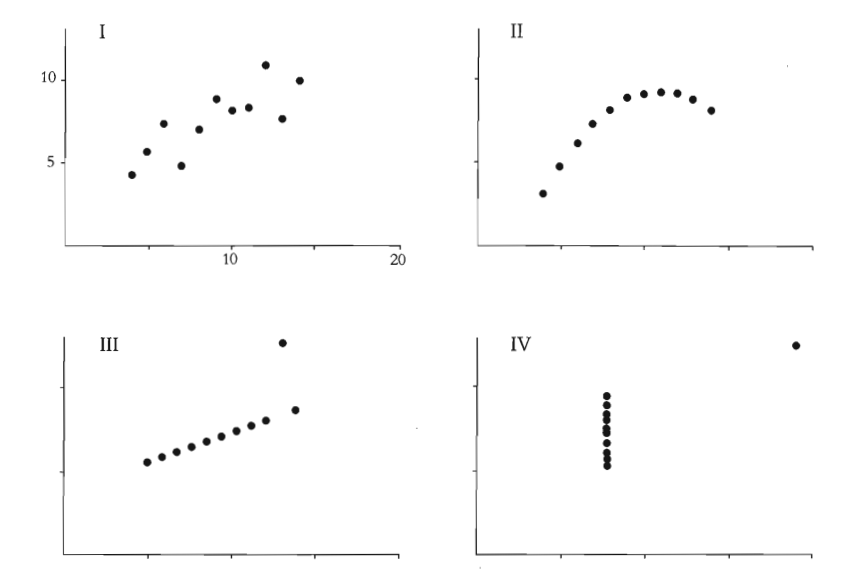
\includegraphics[width=0.8\textwidth,height=\textheight]{excellence_figs/fig_2.png}

Simple statistics fail to exhibit the data trend! Remember to always
visualize!
\end{frame}

\begin{frame}{Why visualize? \textcolor{orange}{Anomaly detection}}
\protect\hypertarget{why-visualize-2}{}
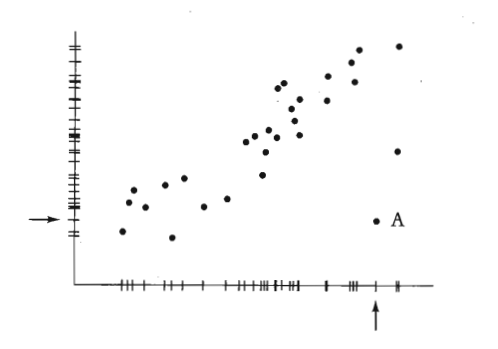
\includegraphics[width=0.8\textwidth,height=\textheight]{excellence_figs/fig_3.png}

Showing the data clearly reveals anomalies.
\end{frame}

\begin{frame}{Data maps}
\protect\hypertarget{data-maps}{}
\begin{minipage}{0.3\textwidth}
\centering
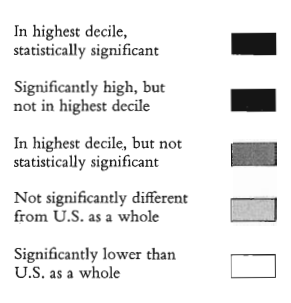
\includegraphics[width=\textwidth]{excellence_figs/fig_5.png}
\end{minipage}
\hfill
\begin{minipage}{0.6\textwidth}
\centering
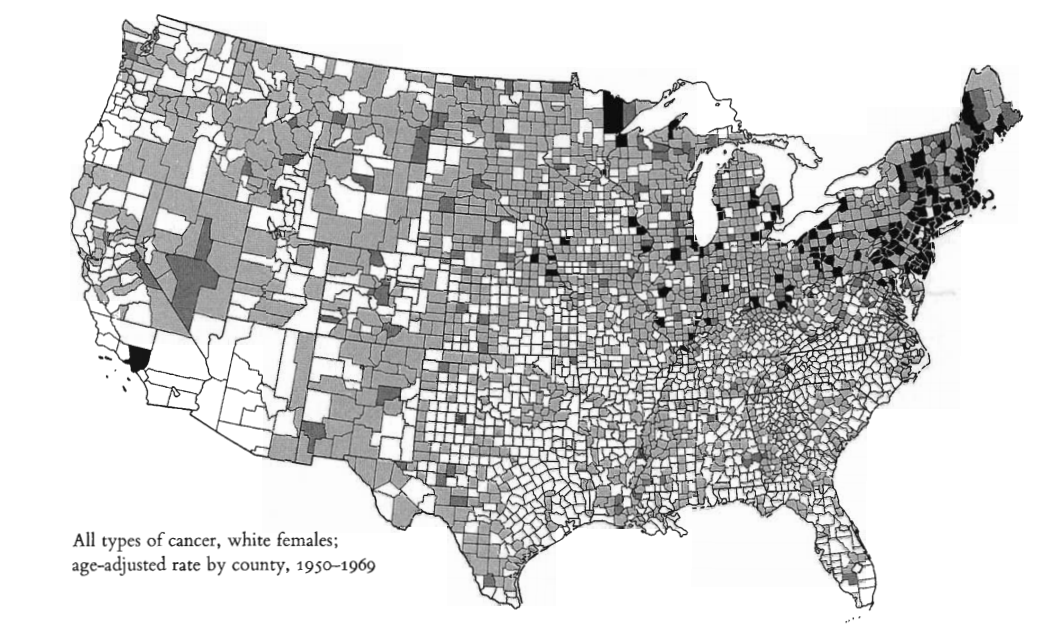
\includegraphics[width=\textwidth]{excellence_figs/fig_4.png}
\end{minipage}

Each map conveys a large amount of information in a small space.

They invite us to search for patterns and to explain their nature.
\end{frame}

\begin{frame}{Data maps}
\protect\hypertarget{data-maps-1}{}
\begin{minipage}{0.3\textwidth}
\centering
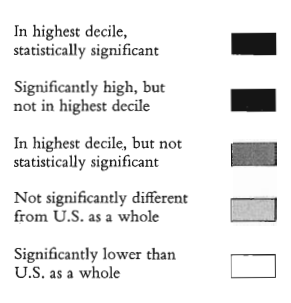
\includegraphics[width=\textwidth]{excellence_figs/fig_7.png}
\end{minipage}
\hfill
\begin{minipage}{0.6\textwidth}
\centering
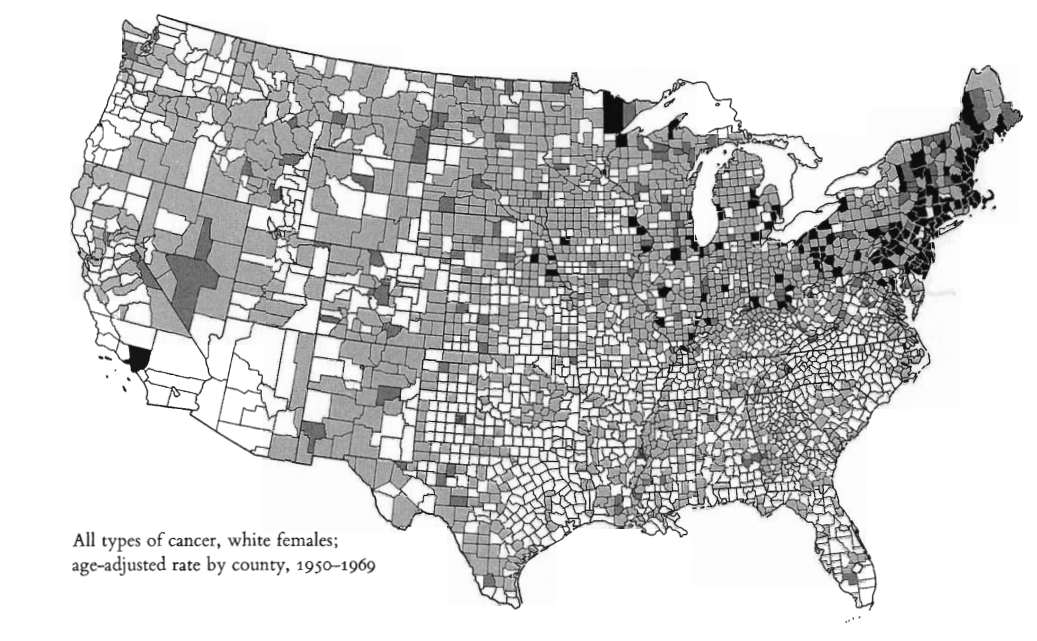
\includegraphics[width=\textwidth]{excellence_figs/fig_6.png}
\end{minipage}

High death rates in the Northeast region and Great Lakes.

Low death rates across central and south bands.
\end{frame}

\begin{frame}{Data maps}
\protect\hypertarget{data-maps-2}{}
\begin{minipage}{0.3\textwidth}
\centering
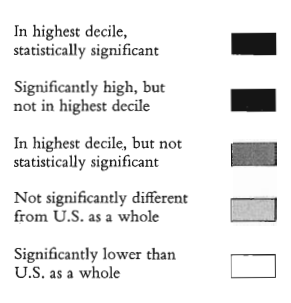
\includegraphics[width=\textwidth]{excellence_figs/fig_9.png}
\end{minipage}
\hfill
\begin{minipage}{0.6\textwidth}
\centering
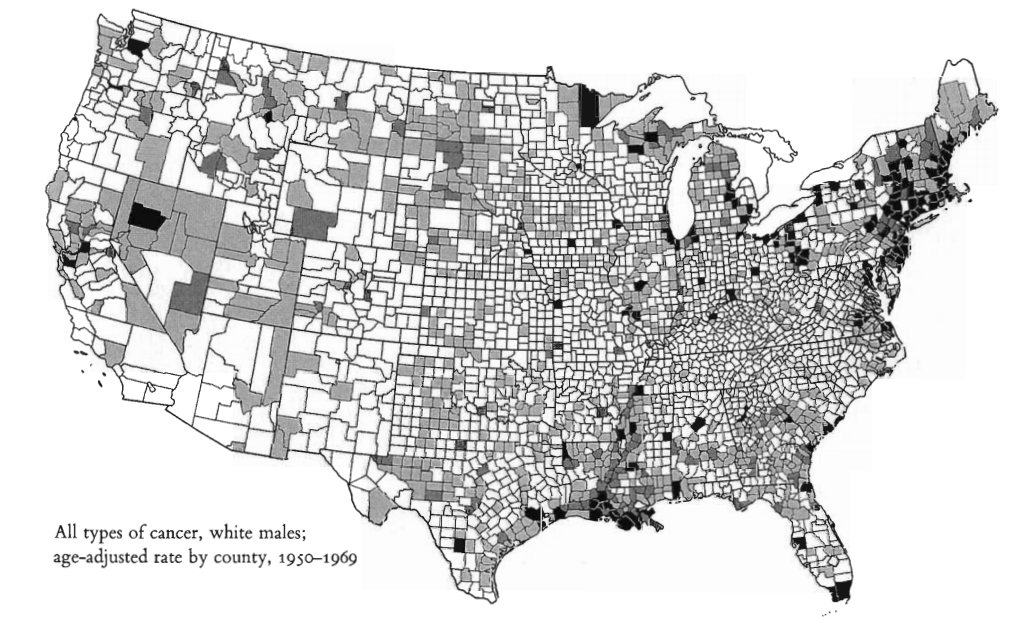
\includegraphics[width=\textwidth]{excellence_figs/fig_10.png}
\end{minipage}

We are now looking at \textcolor{orange}{white males} \ldots{}

Observations?

Explanations?
\end{frame}

\begin{frame}{Data maps}
\protect\hypertarget{data-maps-3}{}
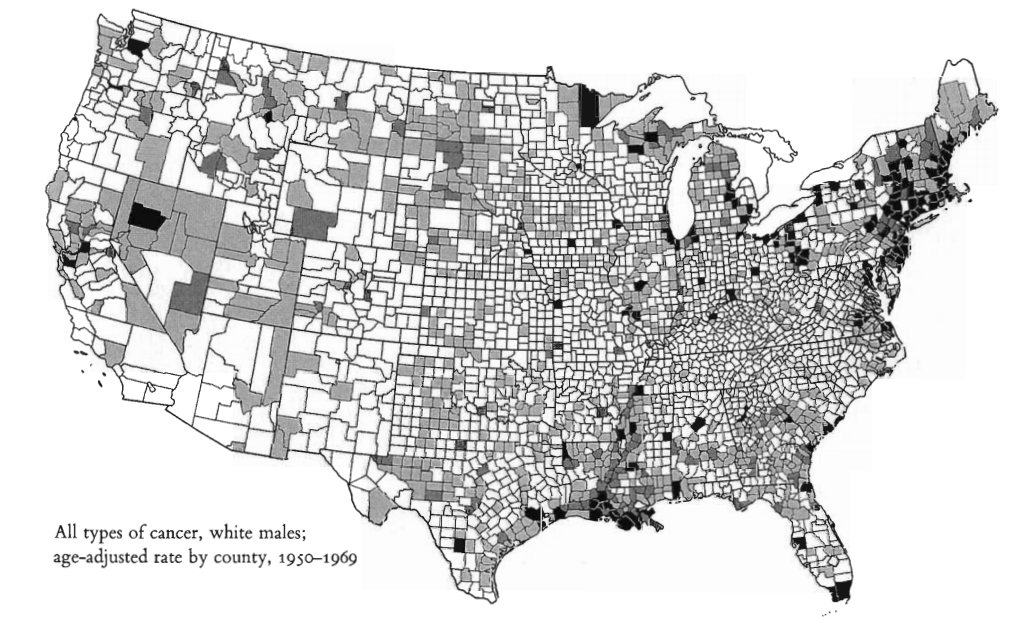
\includegraphics{excellence_figs/fig_10.png}

High death rates in the Louisiana area.
\textcolor{orange}{Asbestos exposure}
\end{frame}

\begin{frame}{Data maps}
\protect\hypertarget{data-maps-4}{}
\textcolor{orange}{Shortcomings}:

\begin{itemize}
\item
  The population of each county is not considered (only area).
\item
  Changes across counties are abrupt (not smooth).
\item
  How reliable is the data? (the diagnosis may be biased).
\end{itemize}
\end{frame}

\begin{frame}{Modern data maps}
\protect\hypertarget{modern-data-maps}{}
\begin{minipage}{0.45\textwidth}
\centering
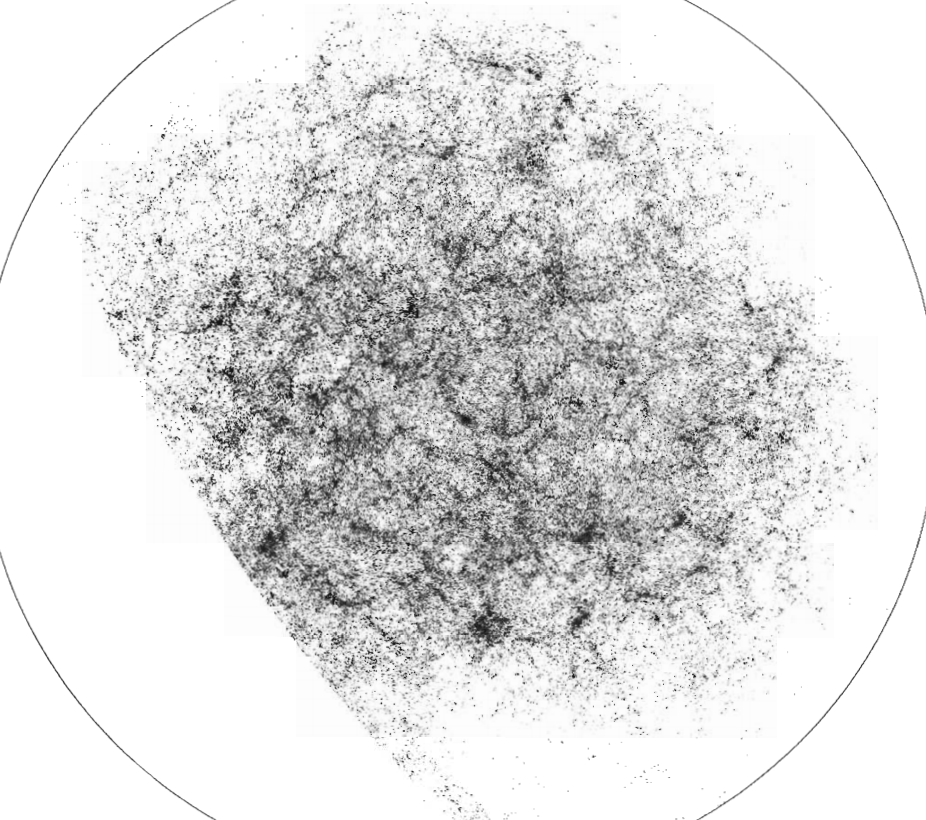
\includegraphics[width=\textwidth]{excellence_figs/fig_12.png}
\end{minipage}
\hfill
\begin{minipage}{0.5\textwidth}
\begin{itemize} \footnotesize
\item Computerized cartography of the universe
\item Distribution of 1.3 million galaxies in the Northern Galactic hemisphere.
\item The darker the gray tone, the more galaxies in that region.
\end{itemize}
\end{minipage}
\end{frame}

\begin{frame}{Time series}
\protect\hypertarget{time-series}{}
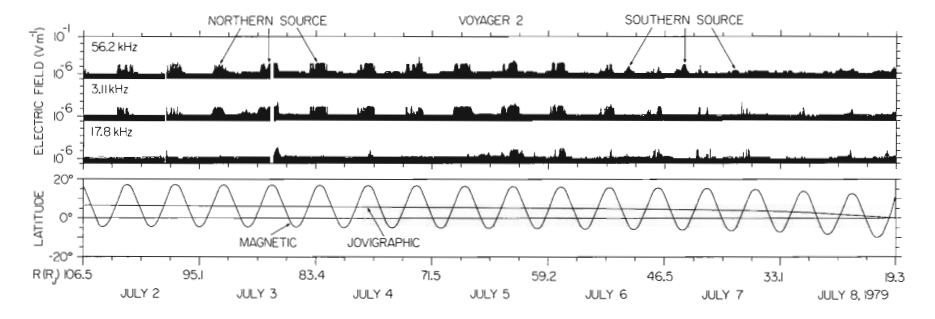
\includegraphics{excellence_figs/fig_13.png}

\begin{itemize}
\item
  This is the most frequent type of graph design.
\item
  The x-axis contains time in one of many possible units (seconds,
  minutes, hours, days, months, years, etc.).
\end{itemize}
\end{frame}

\begin{frame}{Time series}
\protect\hypertarget{time-series-1}{}
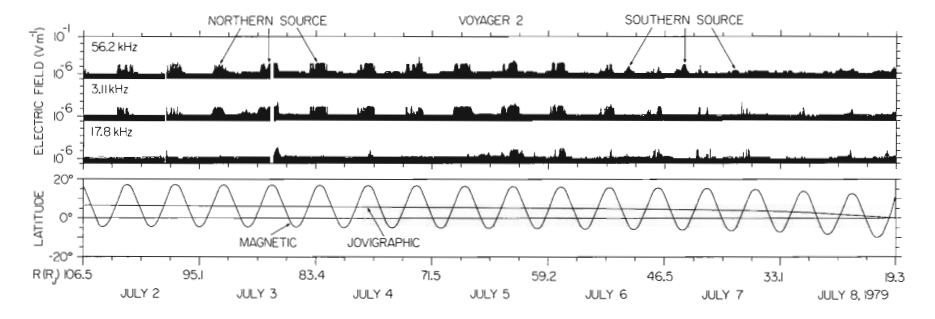
\includegraphics{excellence_figs/fig_14.png}

\begin{itemize}
\item
  Radio emissions from Jupiter captured by Voyager 2 (1979)
\item
  x-axis is both time and distance from Jupiter
\item
  Top three panels are different radio bands
\item
  Bottom panel is orientation of spacecraft
\end{itemize}
\end{frame}

\begin{frame}{Time series}
\protect\hypertarget{time-series-2}{}
\textcolor{orange}{New York City} weather summary (1980)

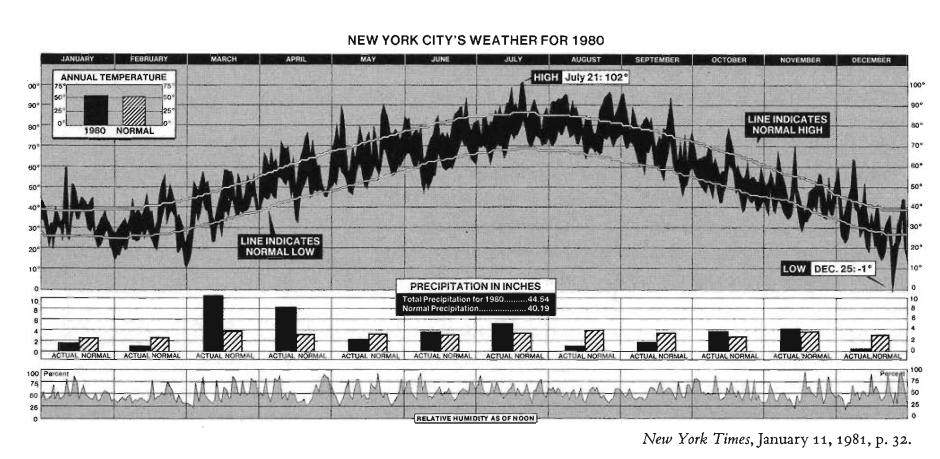
\includegraphics[width=0.95\textwidth,height=\textheight]{excellence_figs/fig_15.png}

How much can you learn from the graph?

The graph tells a story!
\end{frame}

\begin{frame}{Time series}
\protect\hypertarget{time-series-3}{}
Graphical train schedule for Paris to Lyon (1880s).

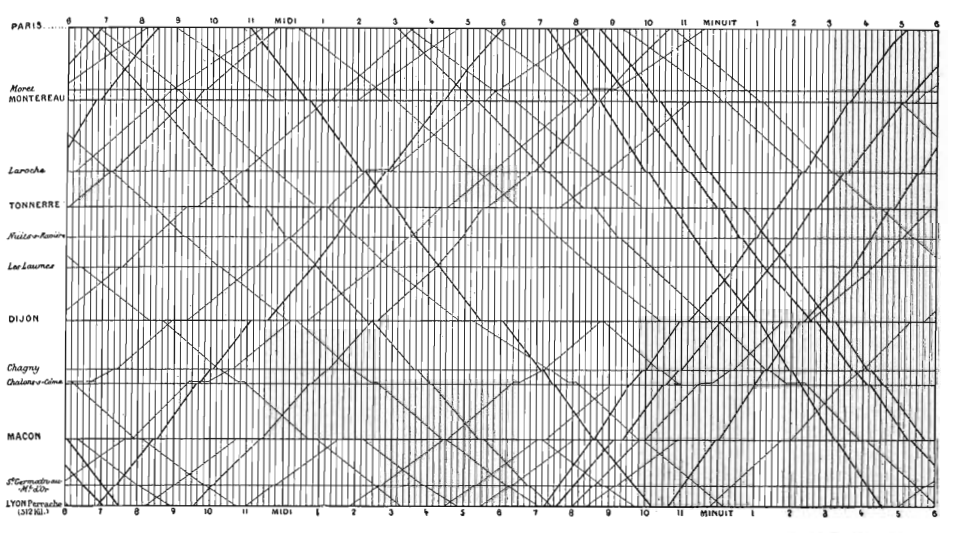
\includegraphics[width=0.9\textwidth,height=\textheight]{excellence_figs/fig_16.png}
\textcolor{orange}{y-axis}: Arrivals/departures, top: Paris, bottom:
Lyon.

\textcolor{orange}{x-axis}: time! Slope of line corresponds to the speed
of the train.
\end{frame}

\begin{frame}{Time series}
\protect\hypertarget{time-series-4}{}
\centering

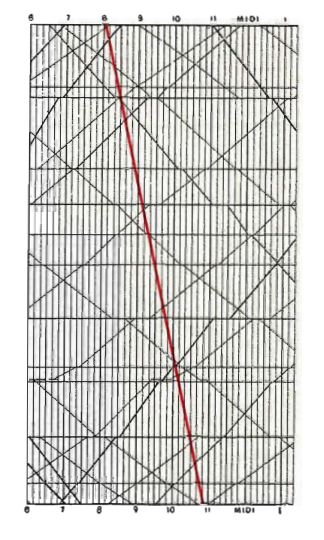
\includegraphics[width=0.4\textwidth]{excellence_figs/fig_17.png}

Extremely fast train came in 1981.
\end{frame}

\begin{frame}{Time series}
\protect\hypertarget{time-series-5}{}
\centering
\begin{minipage}{0.55\textwidth}
\centering
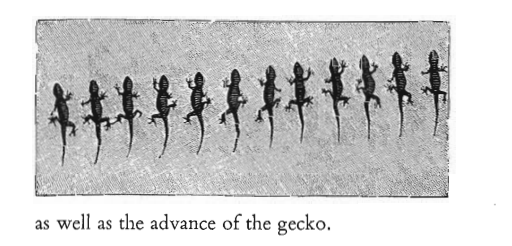
\includegraphics[width=\textwidth]{excellence_figs/fig_19.png}
\end{minipage}
\hfill
\begin{minipage}{0.55\textwidth}
\centering
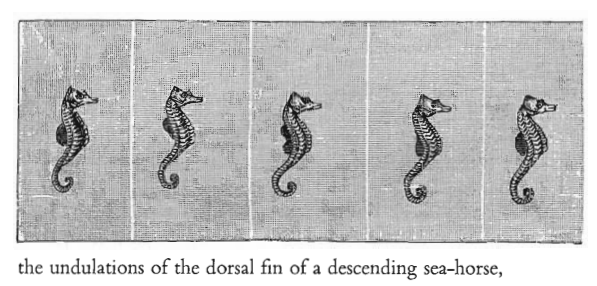
\includegraphics[width=\textwidth]{excellence_figs/fig_18.png}
\end{minipage}

Time series can focus on the graphical evolution of body parts.
\end{frame}

\begin{frame}{Time series}
\protect\hypertarget{time-series-6}{}
\begin{center}
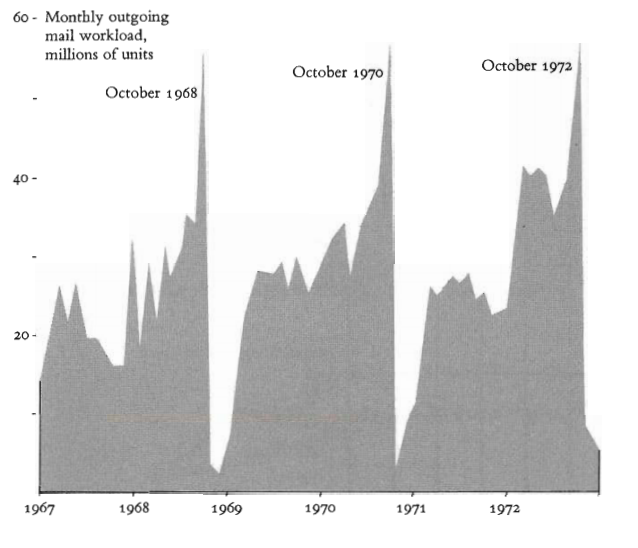
\includegraphics[width=0.55\textwidth]{excellence_figs/fig_20.png}
\end{center}

\footnotesize

Causal information is encoded here \ldots{} how?

Outgoing mail (millions) by incumbent representatives.

Representatives use the privilege of free mail to send many letters
during re-election campaigns.
\end{frame}

\begin{frame}{Space-time narrative designs}
\protect\hypertarget{space-time-narrative-designs}{}
\begin{minipage}{1\textwidth}
\centering
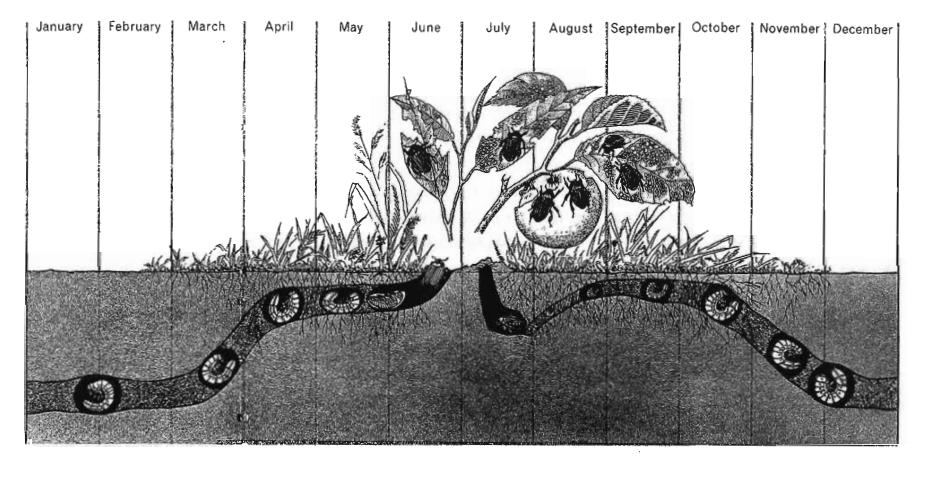
\includegraphics[width=\textwidth]{excellence_figs/fig_21.png}
\end{minipage}
\hfill
\begin{minipage}{1\textwidth}
\footnotesize
\vspace{3mm}
\begin{itemize}
  \item Time-series graphs can be enhanced by adding spatial dimensions.
  \item This adds multivariate complexity that should be easy to visualize and interpret.
  \item Example: Life-cycle of the Japanese beetle.
\end{itemize}
\end{minipage}
\end{frame}

\begin{frame}{Space-time narrative designs}
\protect\hypertarget{space-time-narrative-designs-1}{}
\begin{minipage}{1\textwidth}
\centering
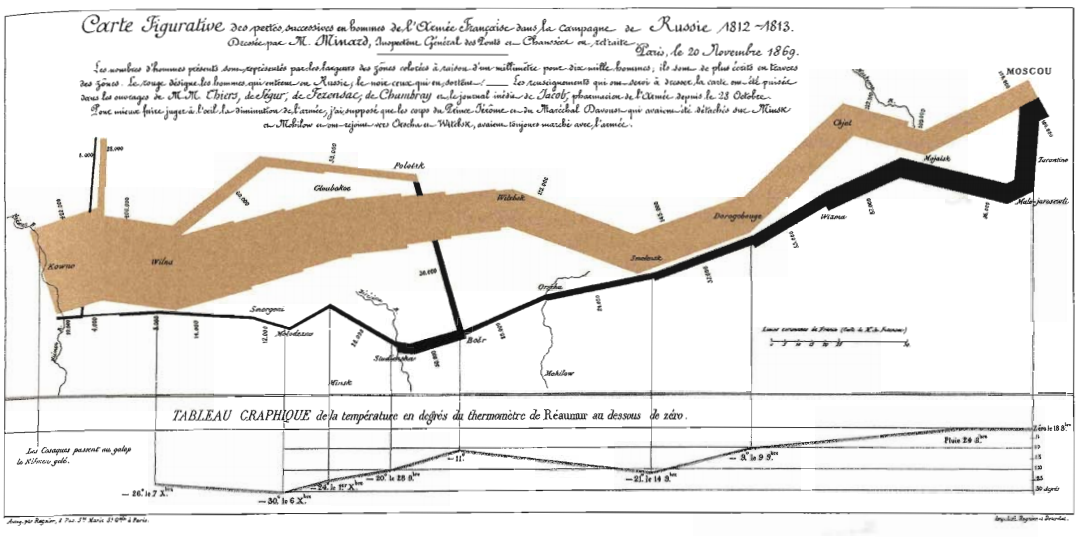
\includegraphics[width=\textwidth]{excellence_figs/fig_22.png}
\end{minipage}
\hfill
\begin{minipage}{1\textwidth}
\footnotesize
\vspace{3mm}
\begin{itemize}
  \item An all-time favorite graph shows the fate of Napoleon's army in Russia (1812-1813).
  \item See the reference book for an explanation.
\end{itemize}
\end{minipage}
\end{frame}

\begin{frame}{Space-time narrative designs}
\protect\hypertarget{space-time-narrative-designs-2}{}
\begin{minipage}{1\textwidth}
\centering
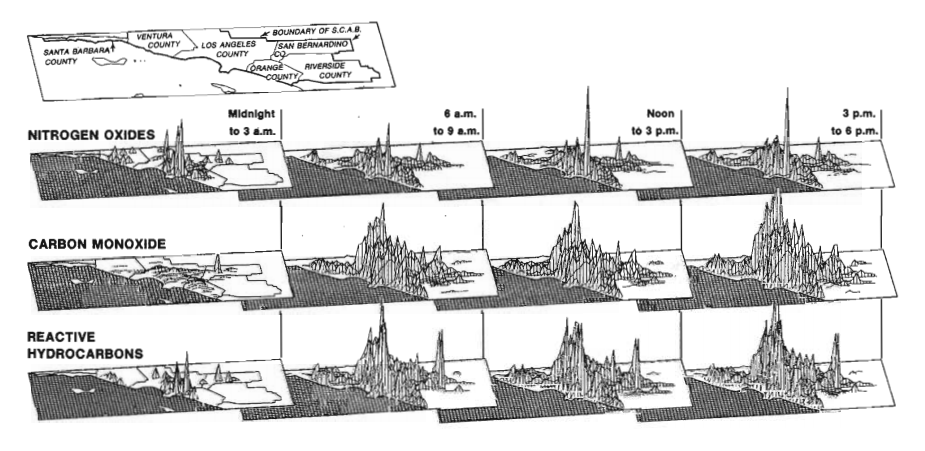
\includegraphics[width=\textwidth]{excellence_figs/fig_23.png}
\end{minipage}
\hfill
\begin{minipage}{1\textwidth}
\footnotesize
\vspace{3mm}
One more example is the levels of air pollutants in southern California during the day.
\end{minipage}
\end{frame}

\begin{frame}{Relational Graphics}
\protect\hypertarget{relational-graphics}{}
\begin{minipage}{1\textwidth}
\centering
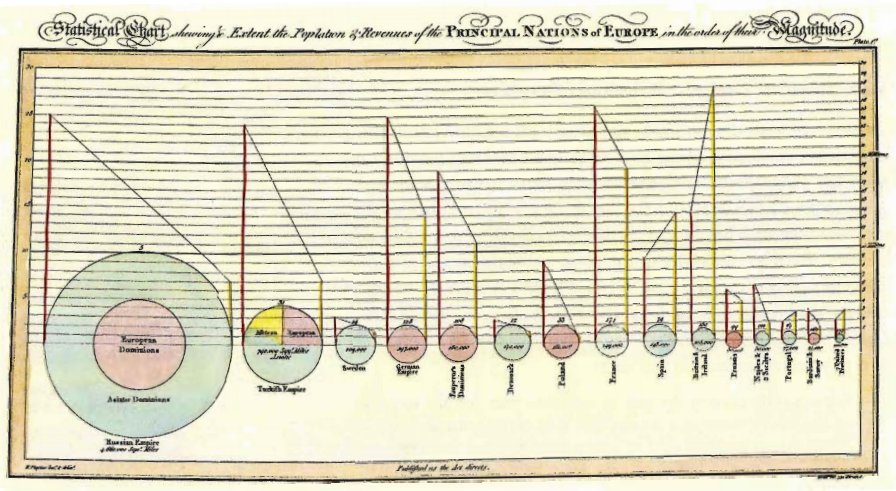
\includegraphics[width=\textwidth]{excellence_figs/fig_24.png}
\end{minipage}
\hfill \vspace{3mm}
\begin{minipage}{1\textwidth}
\footnotesize
\begin{itemize}
  \item Similar to previous graphs, but the dimensions can differ from spatial coordinates.
  \item "Relational" refers to the dependence of two variables (any variables).
\end{itemize}
\end{minipage}
\end{frame}

\begin{frame}{Relational Graphics}
\protect\hypertarget{relational-graphics-1}{}
\begin{minipage}{1\textwidth}
\centering
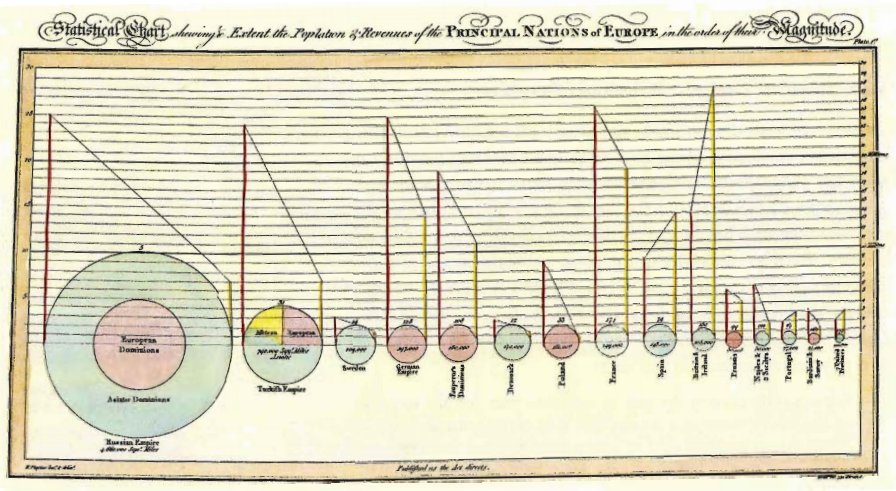
\includegraphics[width=\textwidth]{excellence_figs/fig_24.png}
\end{minipage}
\hfill \vspace{3mm}
\begin{minipage}{1\textwidth}
\footnotesize
\begin{itemize}
  \item Each circle refers to a country, and the size of the circle correlates with the area of the country.
  \item The line on the left is the population in millions, and the line on the right is the taxes collected in millions of pounds.
\end{itemize}
\end{minipage}
\end{frame}

\begin{frame}{Relational graphics}
\protect\hypertarget{relational-graphics-2}{}
\begin{minipage}{0.45\textwidth}
\centering

\includegraphics[width=\textwidth]{excellence_figs/fig_25.png}
\end{minipage}
\hfill
\begin{minipage}{0.5\textwidth}
\footnotesize
\begin{itemize}
  \item Relational graphs are the greatest of graphical designs.
  \item They help look for causal information.
  \item Example: The relationship of lung cancer and smoking.
\end{itemize}
\end{minipage}
\end{frame}

\begin{frame}{Relational graphics}
\protect\hypertarget{relational-graphics-3}{}
\begin{minipage}{0.45\textwidth}
\centering
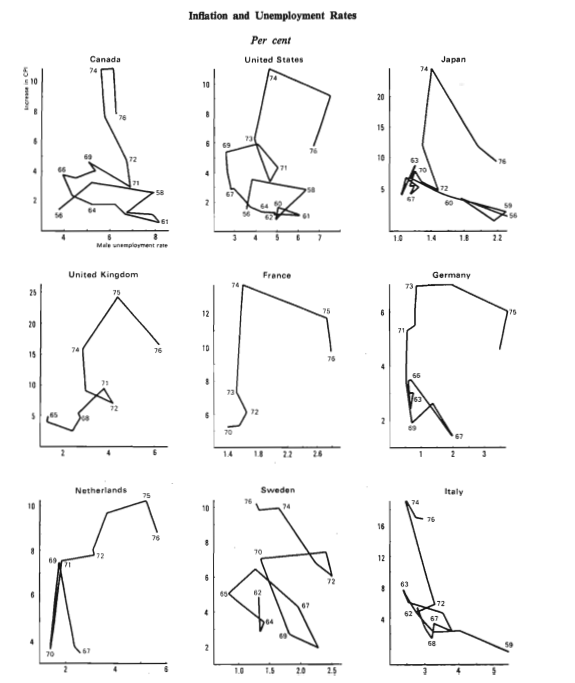
\includegraphics[width=\textwidth]{excellence_figs/fig_26.png}
\end{minipage}
\hfill
\begin{minipage}{0.5\textwidth}
\footnotesize
\begin{itemize}
  \item Relational graphs are the greatest of graphical designs.
  \item They help look for causal information.
  \item Is there a connection between inflation and unemployment?
  \item Apparently NOT!
\end{itemize}
\end{minipage}
\end{frame}

\begin{frame}{Relational graphics}
\protect\hypertarget{relational-graphics-4}{}
\begin{minipage}{0.45\textwidth}
\centering
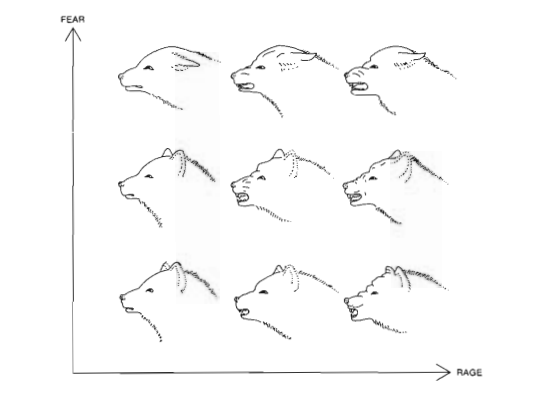
\includegraphics[width=\textwidth]{excellence_figs/fig_27.png}
\end{minipage}
\hfill
\begin{minipage}{0.5\textwidth}
\footnotesize
\begin{itemize}
  \item Relational Graphics
  \item Graphs can be very informative.
  \item Data points can convey a lot of information.
  \item Rage (x-axis) vs Fear (y-axis).
\end{itemize}
\end{minipage}
\end{frame}

\begin{frame}{Summary}
\protect\hypertarget{summary}{}
\begin{minipage}{0.45\textwidth}
\centering
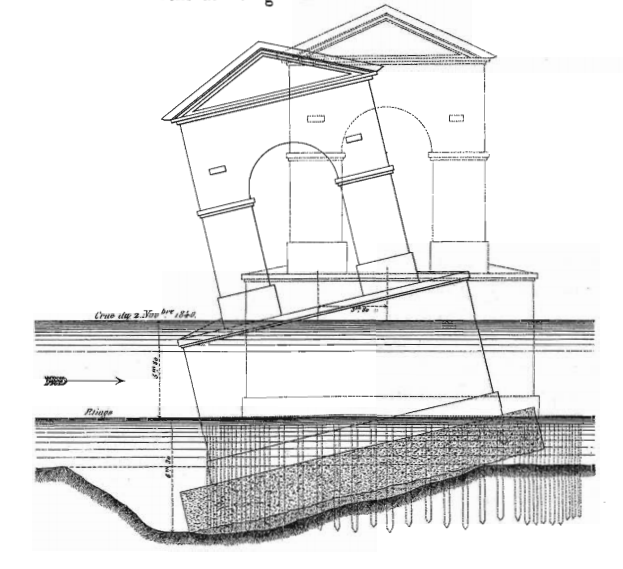
\includegraphics[width=\textwidth]{excellence_figs/fig_35.png}
\end{minipage}
\hfill
\begin{minipage}{0.5\textwidth}
\footnotesize
\begin{itemize}
  \item Good graphs succinctly convey substantial information.
  \item Coming up with a good design is challenging.
  \item Ideas must be conveyed with clarity, precision, and efficiency.
\end{itemize}
\end{minipage}
\end{frame}

\end{document}
